\documentclass[12pt]{beamer}

% Presento style file
\usepackage{config/presento}
\usepackage{enumitem}
\setitemize{label=\usebeamerfont*{itemize item}%
    \usebeamercolor[colorgreen]{itemize item}
    \usebeamertemplate{itemize item}}
    
% custom command and packages
% custom packages
\usepackage{textpos}
\setlength{\TPHorizModule}{1cm}
\setlength{\TPVertModule}{1cm}

\newcommand\crule[1][black]{\textcolor{#1}{\rule{2cm}{2cm}}}



% Information
\title{Eternity Calculator}
\subtitle{Project Organization \& Summary}
\author{Team I}
\institute{COMP 354 - Summer 2021}
\date{June 11, 2021}

\begin{document}

% Title page
\begin{frame}[plain]
\maketitle
\end{frame}

% sections in the presentation
\begin{frame}{Table of Contents}
  \item {\notosansfont 1. Initial Project Meeting}
  \itemsep1em
  \item {\notosansfont 2. Roles}
  \item {\notosansfont 3. GitHub Repository}
  \item {\notosansfont 4. Interview Process}
  \item {\notosansfont 5. Personas}
  \item {\notosansfont 6. Use Cases}
  \item {\notosansfont 7. Conclusion}
\end{frame}

% Initial Project Meeting
\begin{frame}{Initial Project Meeting}
 \begin{fullpageitemize}
    \item Decision of the technology and language for Eternity \pause
    \item Breakdown of team members' skills, tasks and responsibilities \pause
    \item Organization of future meetings and communication
    \begin{itemize}
        \item Discord 
    \end{itemize}
     \begin{figure}
     \centering
     
\includegraphics[width=0.25\textwidth]{images/discord.png}       \end{figure}
 \end{fullpageitemize}
\end{frame}

% Project Breakdown
\begin{frame}{Project Breakdown}
 \begin{fullpageitemize}
    \item Leader - Project and repository organizer
    \item Documentation
    \item Full-stack Developer
    \item Back-end Developer
    \item Front-end Developer
    \item Communication and resources
 \end{fullpageitemize}
\end{frame}

% Roles
\begin{frame}{Roles}
    \item \textcolor{colorgreen}{Leader:} Robert
    \itemsep1em
    \item \textcolor{colorgreen}{Documentation:} Xavier, Sobhan
    \item \textcolor{colorgreen}{Full-stack Developer:} Chelsie 
    \item \textcolor{colorgreen}{Back-end Developer:} Elijah
    \item \textcolor{colorgreen}{Front-end Developer:} Michael
    \item \textcolor{colorgreen}{Communication and resources:} Hao Mei
    \item \textcolor{colorgreen}{Major presenter:} Michael
    \item \textcolor{colorgreen}{Minor presenter:} Robert
\end{frame}

% GitHub Repository
\begin{frame}{GitHub Repository}
    \begin{figure}
     \centering
     
\includegraphics[width=0.25\textwidth]{images/github.png}       \end{figure}
    \item More than a code hosting platform for version control: \pause
    \begin{itemize}
        \item Issue tracking \pause
        \itemsep1em
        \item Kanban board linked to current issues \pause
        \item Documentation - wiki
    \end{itemize}
\end{frame}

% Issues
\begin{frame}{GitHub Issues}
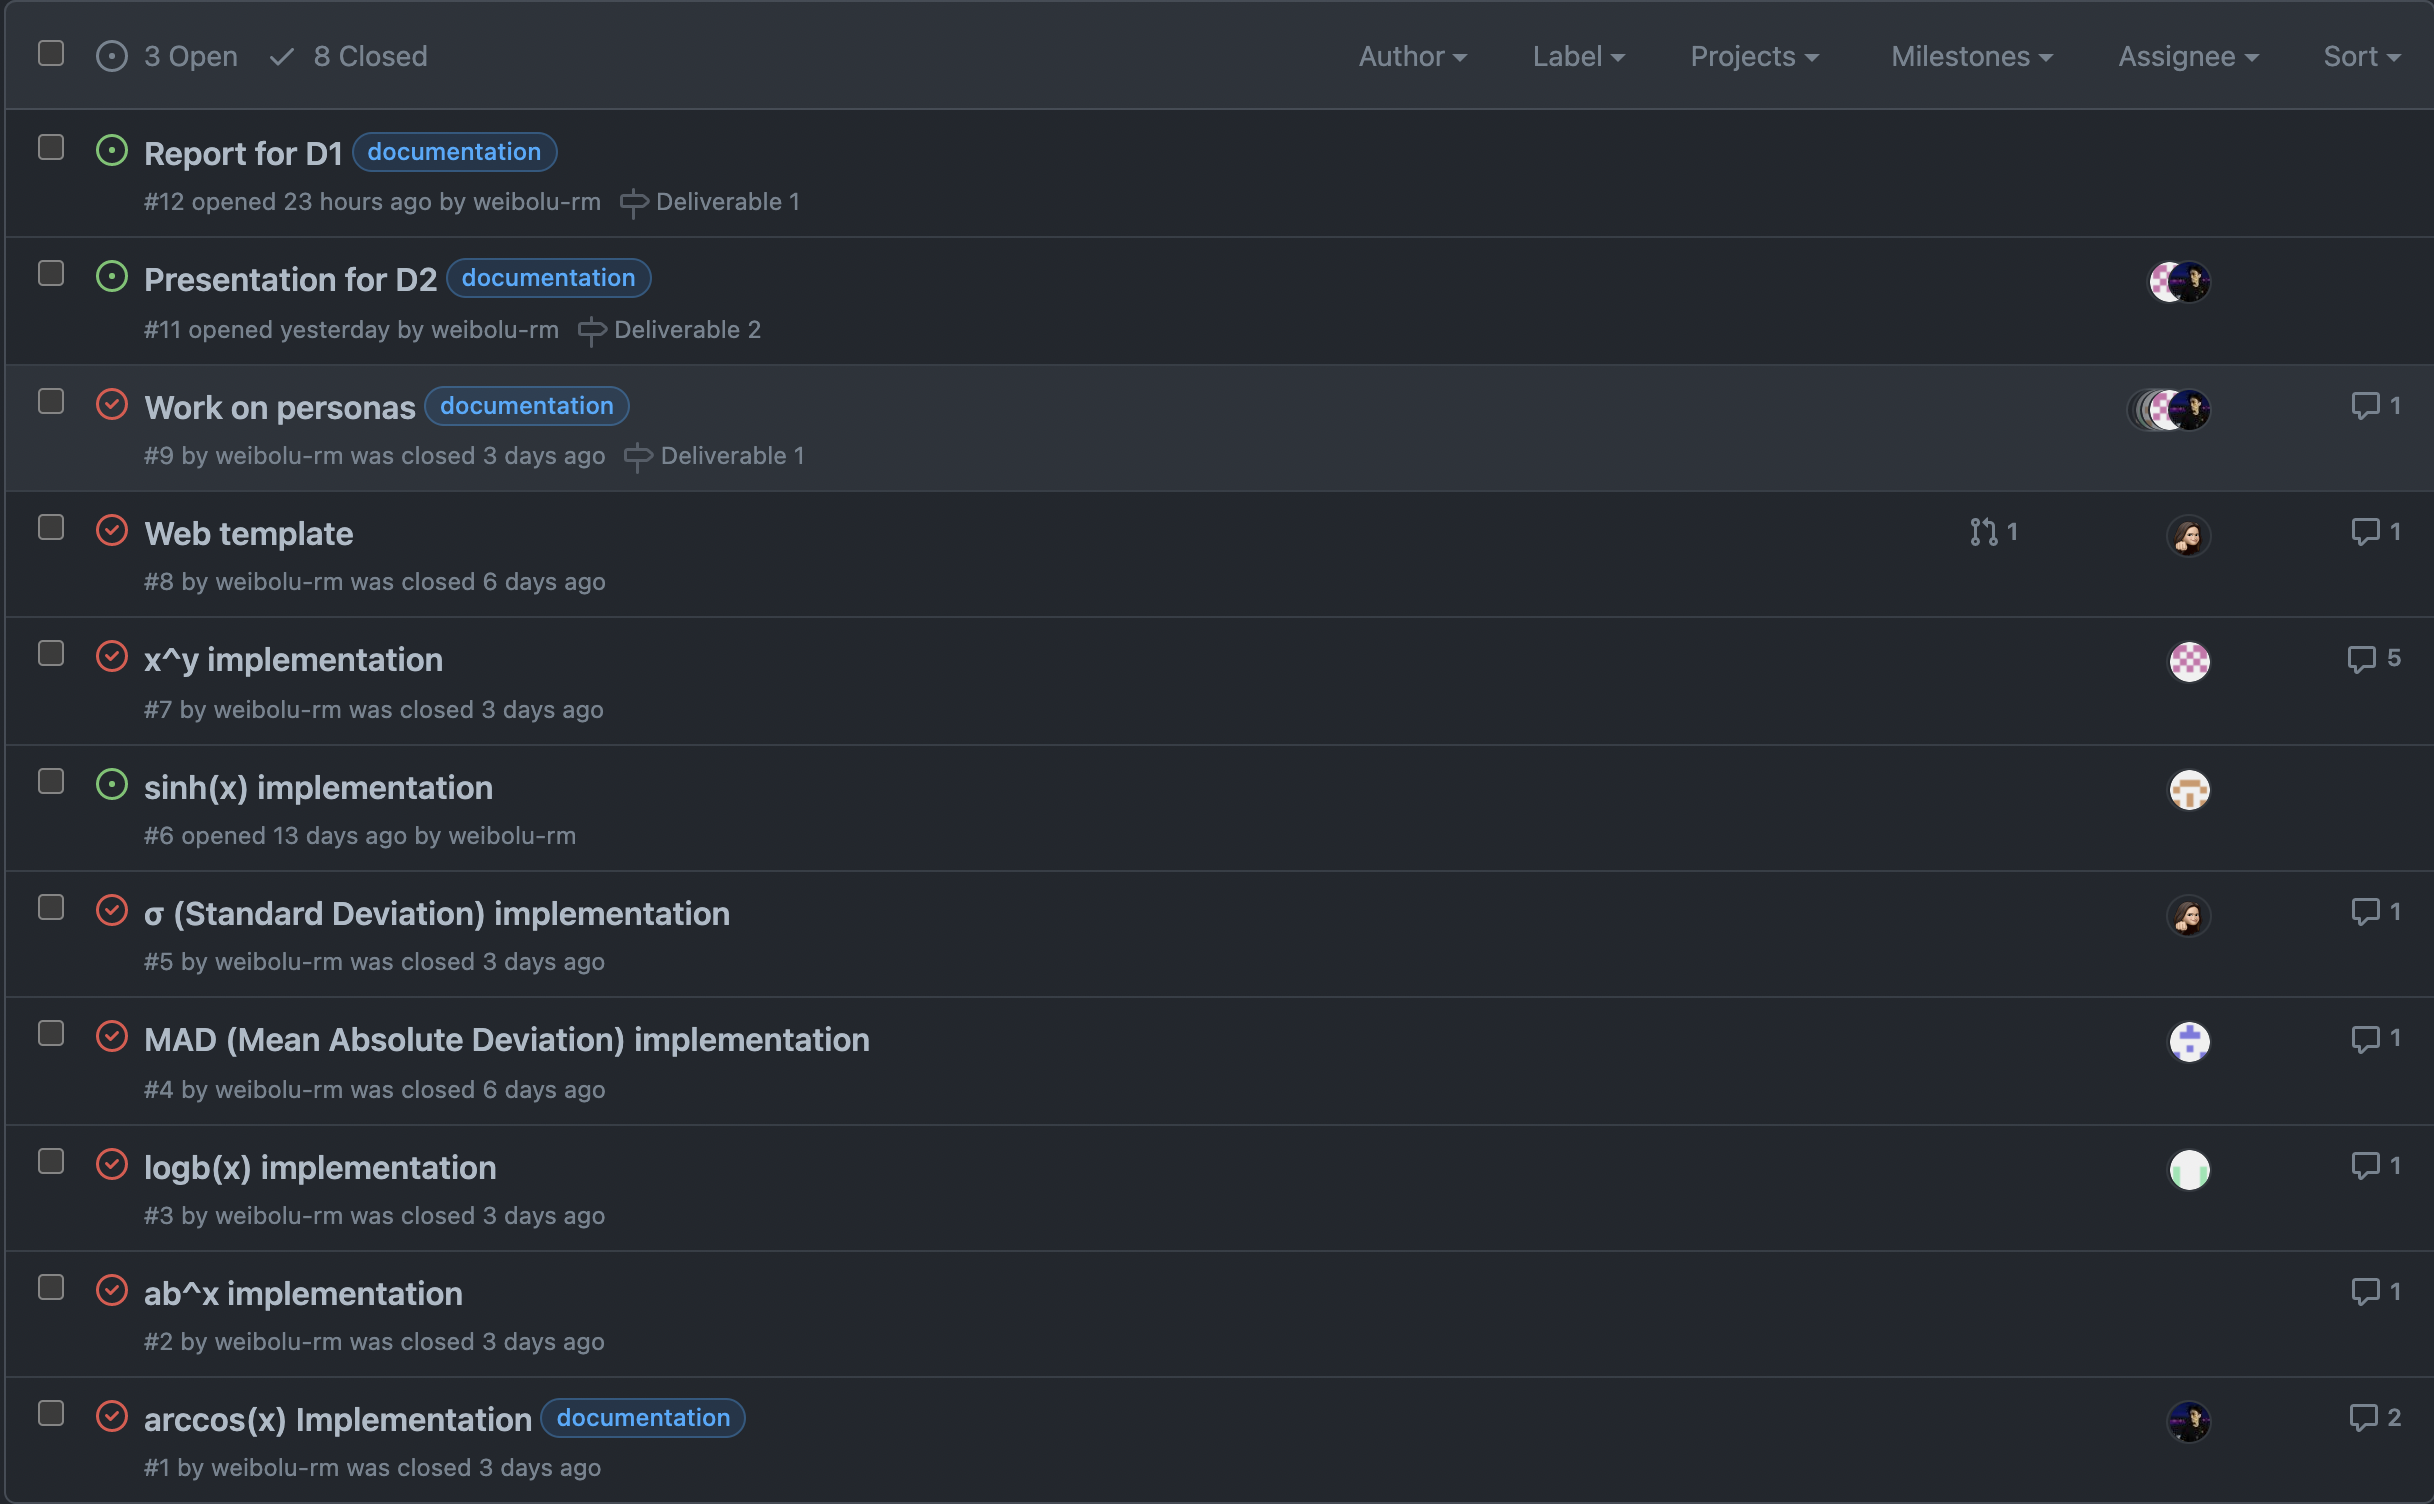
\includegraphics[width=1\linewidth]{images/issues.png}
\end{frame}

% Kanban board
\begin{frame}{Kanban Board}
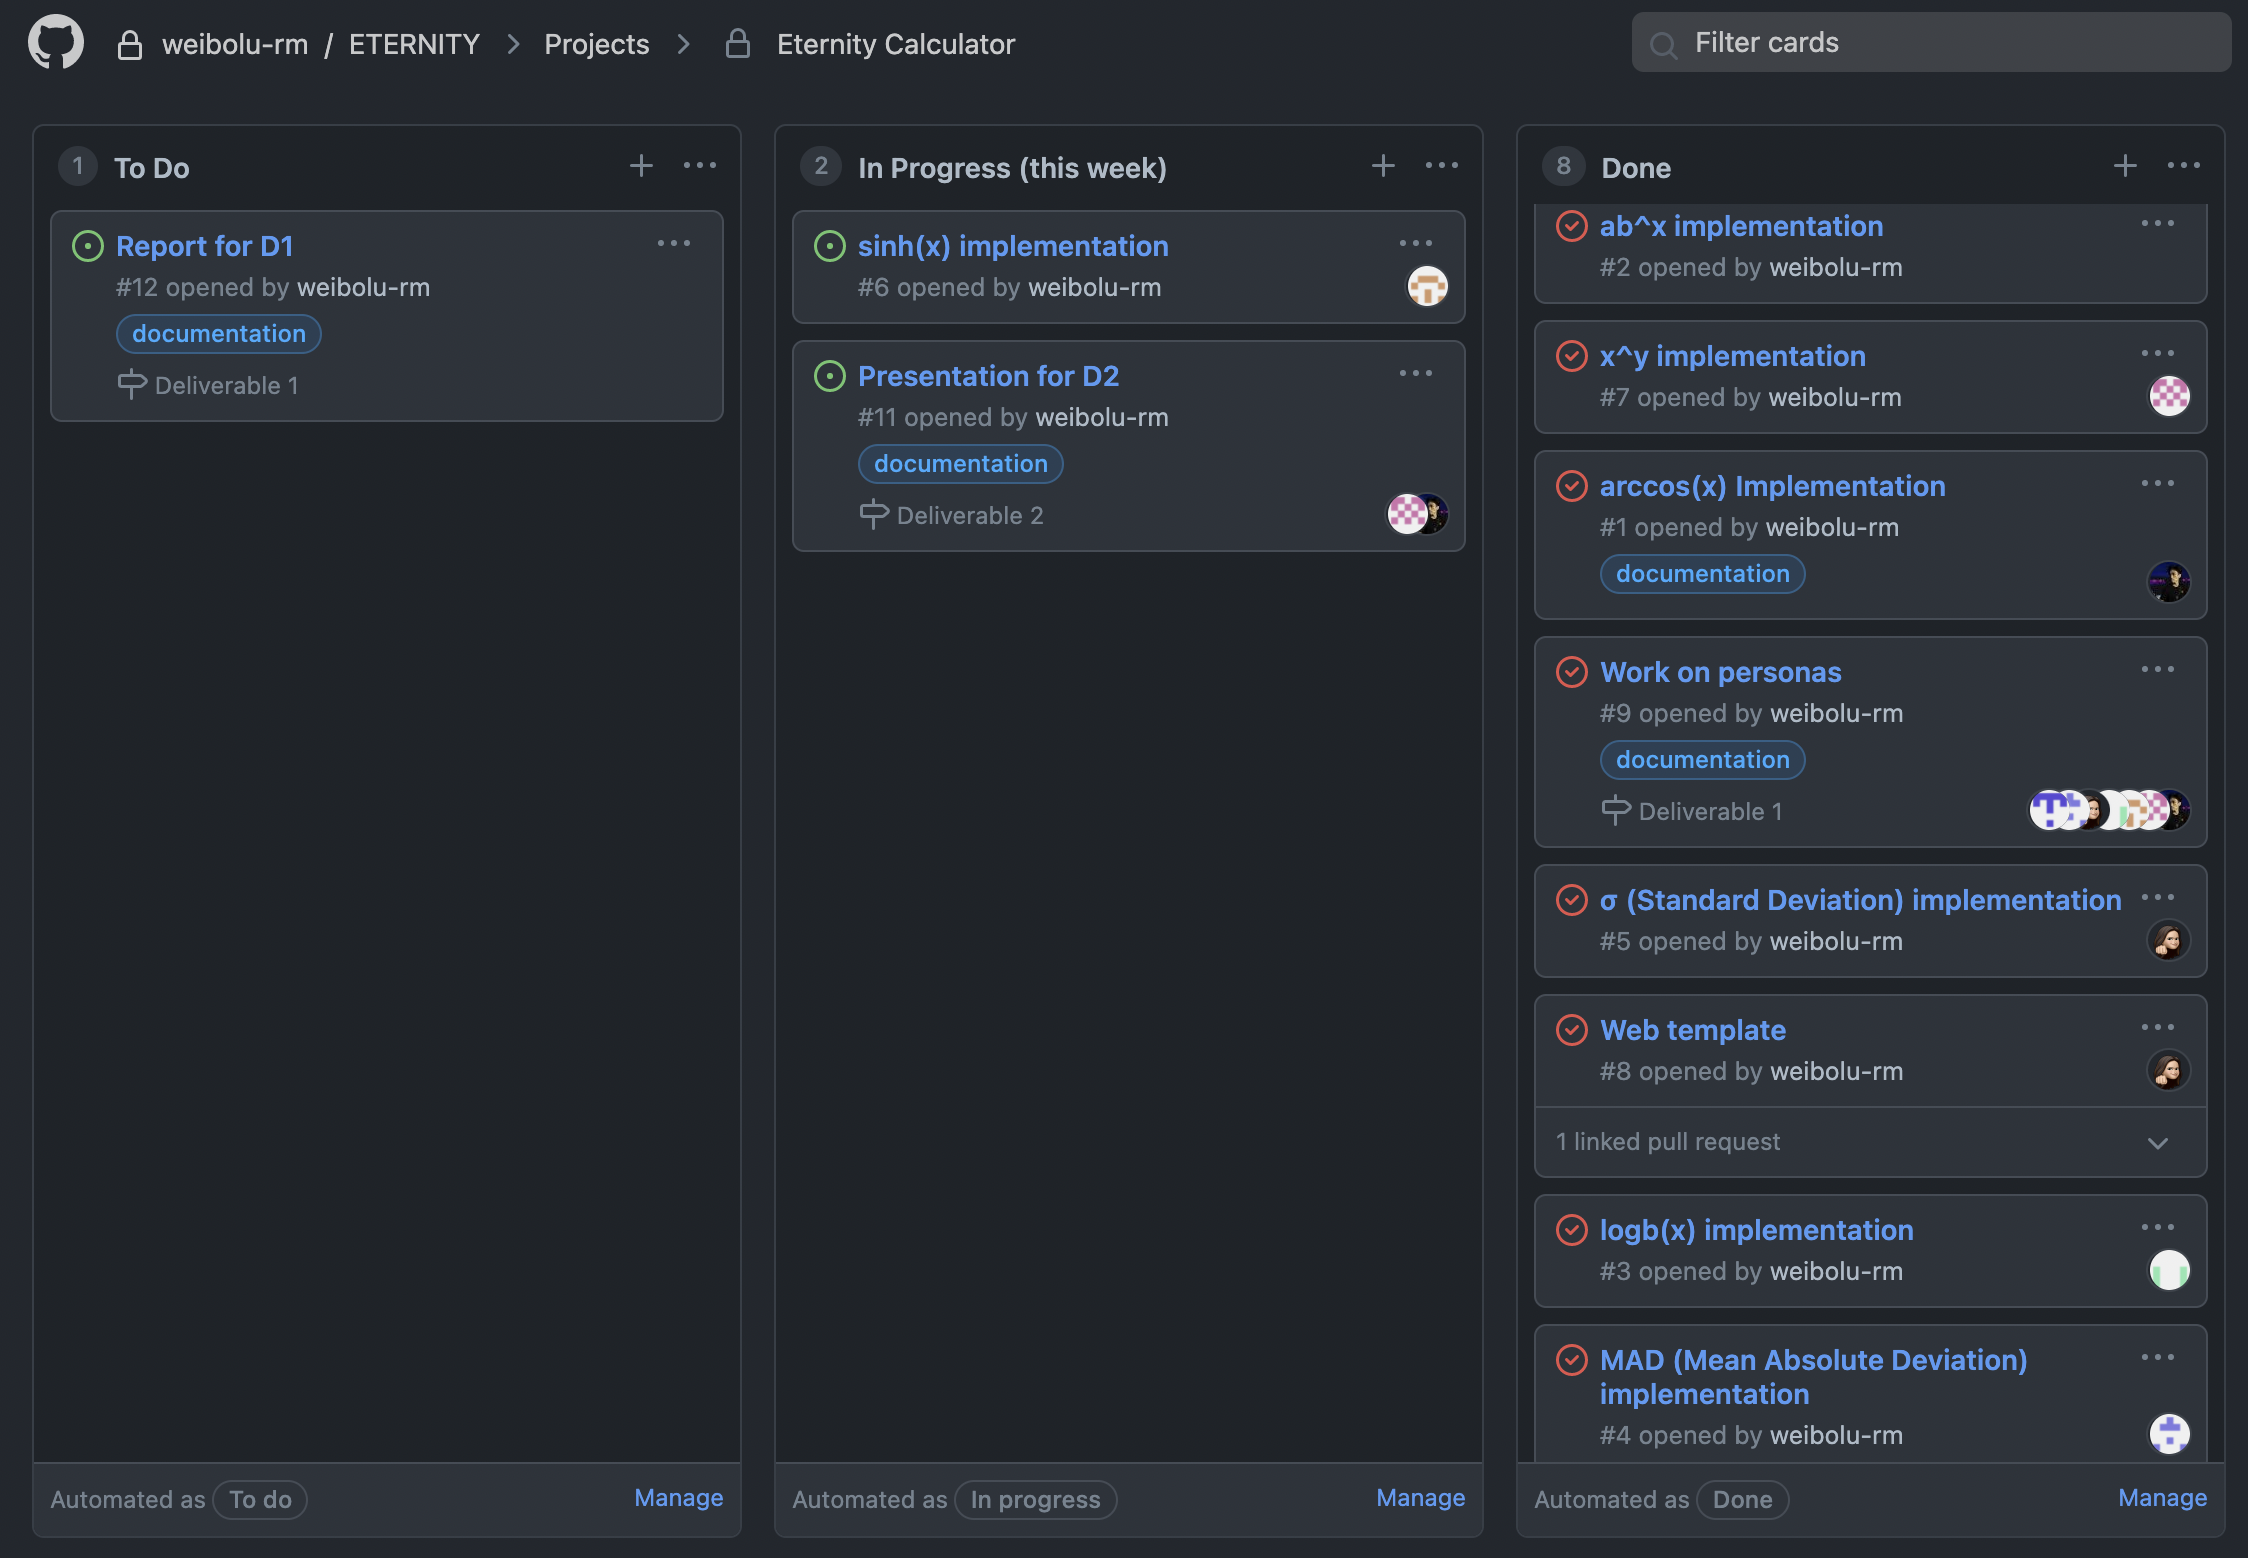
\includegraphics[width=1\linewidth]{images/kanban.png}
\end{frame}

% Documentation
\begin{frame}{Wiki}
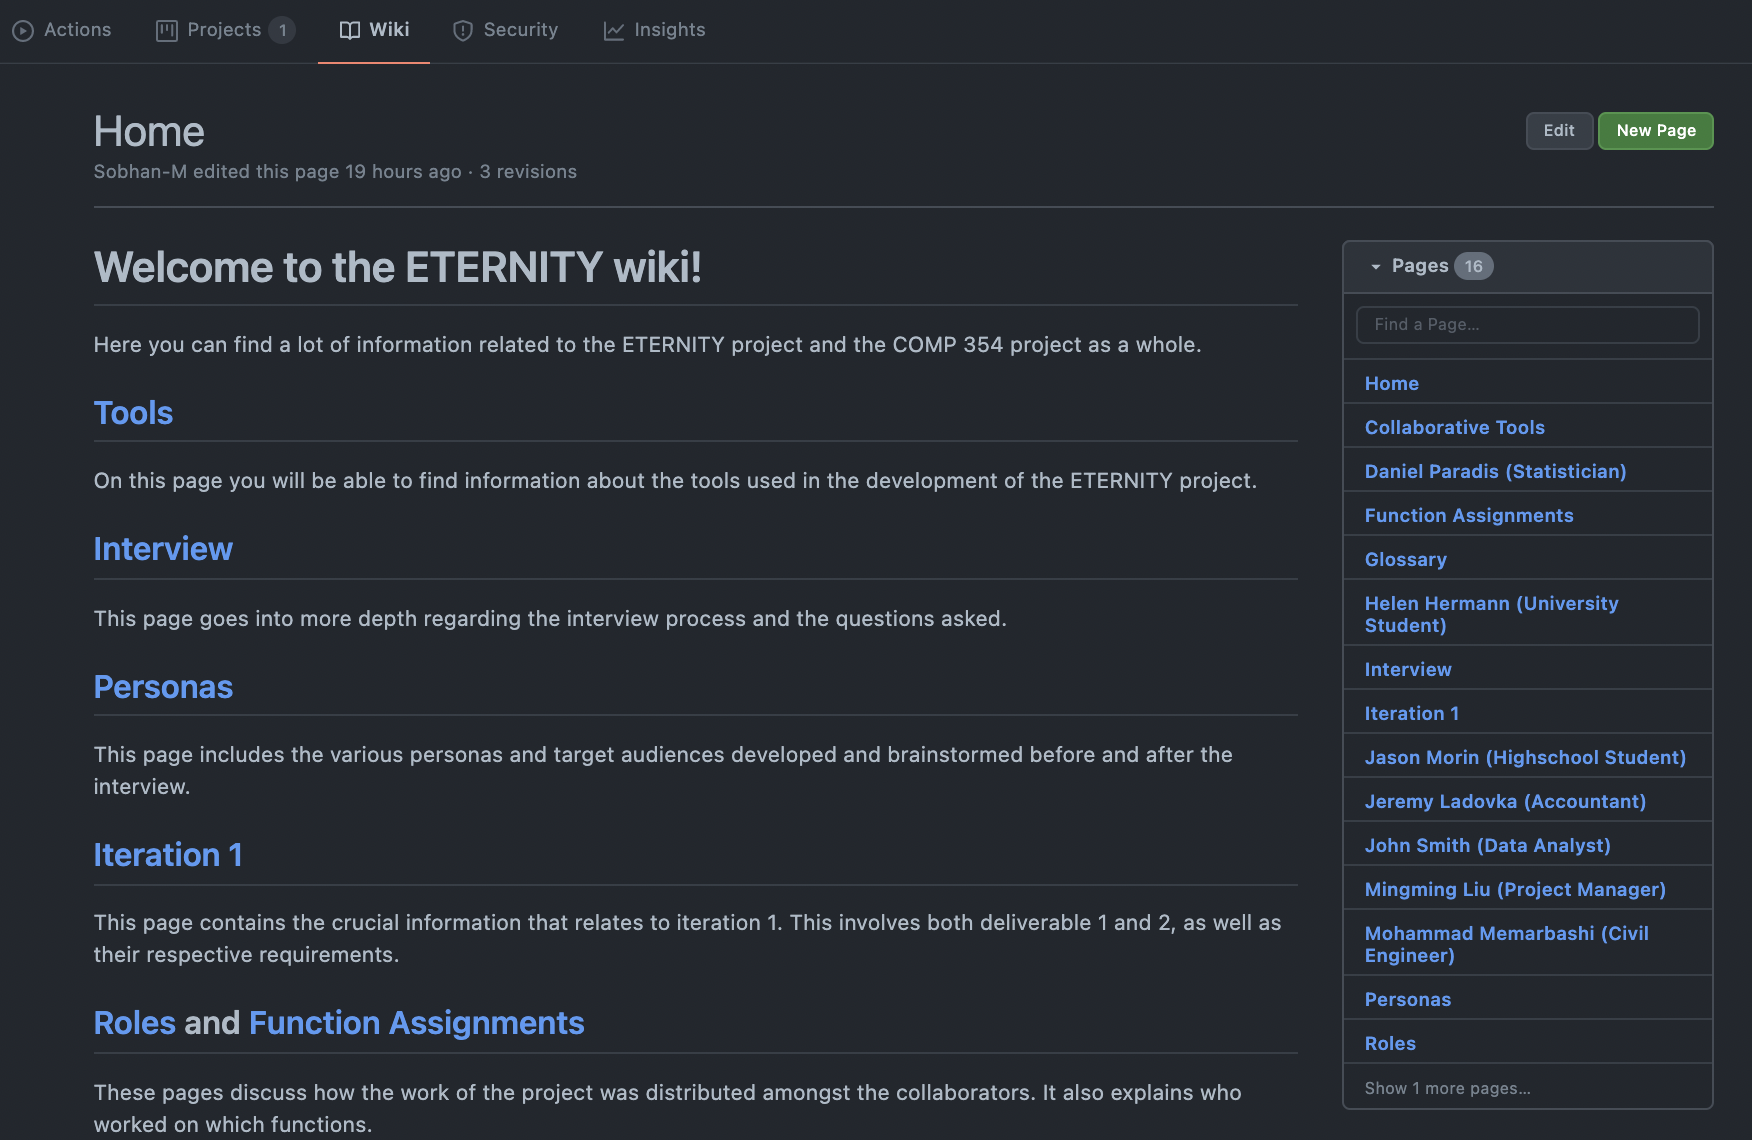
\includegraphics[width=1\linewidth]{images/wiki.png}
\end{frame}

% Interview Process
\begin{frame}{Interview Process}
 \begin{fullpageitemize}
  \item Funnel Strategy 
    \begin{itemize}
        \item General questions leading into more specific questions related to the calculator. \pause
    \end{itemize}
    \itemsep1em
  \item Semi-structured \& Linear Progression 
    \begin{itemize}
        \item Asked some follow-up sub-questions based on the response to get more information
        \item General questions to increasingly more specific questions (Funnel Strategy) \pause
    \end{itemize}
  \item 5 questions per team member
  \begin{itemize}
        \item 10 General questions
        \item 25 Specific questions
    \end{itemize}
 \end{fullpageitemize}
\end{frame}

% Choosing Interviewees
\begin{frame}{Choosing Interviewees}
 \begin{fullpageitemize}
    \item Aimed for a variety of interviewees based on whom we thought would be interested in using a calculator \pause
    \item Total of 7 interviewees, one interview conducted by each team member
 \end{fullpageitemize}
\end{frame}

% Main takeaways from interview
\begin{frame}{Main takeaways}
 \begin{fullpageitemize}
    \item Customizability \pause
    \item Preference of formal notation \\ i.e. \textit{x^y \ vs \ x \textasciicircum y\\} \pause
    \item Existence of few popular online calculators/ tools with advanced features \\ i.e. \textit{WolframAlpha, Symbolab, Desmos\\}
 \end{fullpageitemize}
\end{frame}

% Example of an idea we didn't consider
\begin{frame}{Example of a \underline{discarded} idea }
    \item \textcolor{colorgreen}{Which functions that are generally not on a calculator, would you like to see added?} \pause
    \itemsep1em
    \item "This is very difficult, maybe some constants could be added, like the gravity constant or the speed of light for our fellow engineers."
\end{frame}

% Initial Personas
\begin{frame}{Initial Personas}
    \item People ranging from different backgrounds who might 
    contribute to different types of use cases: 
    \itemsep1em
    \item \textcolor{colorgreen}{1.} Students
    \item \textcolor{colorgreen}{2.} Statisticians
    \item \textcolor{colorgreen}{3.} Data Analysts
    \item \textcolor{colorgreen}{4.} Businessmen
    \item \textcolor{colorgreen}{5.} Accountants
    \item \textcolor{colorgreen}{6.} Engineers
    \item \textcolor{colorgreen}{7.} Professors
\end{frame}

% Target Personas
\begin{frame}{Actual Target Personas}
    \item \textcolor{colorgreen}{1.} High-school Student
    \itemsep1em
    \item \textcolor{colorgreen}{2.} University Student
    \item \textcolor{colorgreen}{3.} Statistician
    \item \textcolor{colorgreen}{4.} Data Analyst
    \item \textcolor{colorgreen}{5.} Accountant
    \item \textcolor{colorgreen}{6.} Engineer (Program Manager)
    \item \textcolor{colorgreen}{7.} Civil Engineer
\end{frame}

% Personas Overview 
\begin{frame}{Personas Overview}
    \item Using the interview responses: \pause
    \itemsep1em
    \item
    \begin{itemize}
        \item Wrote up a basic bio to make it more "real" \pause
        \itemsep1em
        \item Came up with positive and negative personas \pause
        \item Built a table with important information
    \end{itemize}
\end{frame}

% Persona for the target group "High-school Student"
\begin{frame}{High-school Student}
    \resizebox{1\textwidth}{!}{%
    \begin{tabular}{ ll } 
        \hline
        \textcolor{colorgreen}{Name}                          & Jason Morin                          \\ \hline
        \textcolor{colorgreen}{Gender and Age}                & Male, 15                             \\ \hline
        \textcolor{colorgreen}{Disabilities and restrictions} & None                                 \\ \hline
        \textcolor{colorgreen}{Education}                     & Current high-school student          \\ \hline
        \textcolor{colorgreen}{Profession}                    & Student                              \\ \hline
        \textcolor{colorgreen}{Hobbies}                       & Building (customizing) computers,    \\ 
                                                              & video games, watching Netflix        \\ \hline
        \textcolor{colorgreen}{Location of use}               & Home                                 \\ \hline
                                                              & Very comfortable using computers,    \\
        \textcolor{colorgreen}{Computer literacy}             & and a fast learner for new programs/ \\
                                                              & tools but not a power user.          \\ \hline
        \textcolor{colorgreen}{Computer environment}          & \textit{Google Chrome 91.0.4472.77}  \\ 
                                                              & on \textit{Windows 10}               \\ \hline
        \textcolor{colorgreen}{Internet literacy}             & High, self-taught and fast learner   \\ \hline
    \end{tabular}%
    }
\end{frame}

% Persona for the target group "Accountant"
\begin{frame}{Accountant}
    \resizebox{1\textwidth}{!}{%
    \begin{tabular}{ ll } 
        \hline
        \textcolor{colorgreen}{Name}                          & Jeremy Ladovka                        \\ \hline
        \textcolor{colorgreen}{Gender and Age}                & Male, 38                              \\ \hline
        \textcolor{colorgreen}{Disabilities and restrictions} & None                                  \\ \hline
        \textcolor{colorgreen}{Education}                     & Masters, Accountancy                  \\ \hline
        \textcolor{colorgreen}{Profession}                    & Accountant                            \\ \hline
        \textcolor{colorgreen}{Hobbies}                       & Math, soccer, watching movies,        \\ 
                                                              & playing video games, going out        \\
                                                              & with friends                          \\ \hline
        \textcolor{colorgreen}{Location of use}               & Office/Home(COVID-19)                 \\ \hline
                                                              & Very strong computer skills           \\
        \textcolor{colorgreen}{Computer literacy}             & Uses computers on a daily basis       \\ 
                                                              & to perform both work related          \\
                                                              & tasks and personal hobbies.           \\ \hline
        \textcolor{colorgreen}{Computer environment}          & \textit{Google Chrome 91.0.4472.77}   \\ 
                                                              & \textit{Safari v14.1, Mac OS}         \\ \hline
        \textcolor{colorgreen}{Internet literacy}             & High, communicates via Internet daily \\ \hline
    \end{tabular}%
    }
\end{frame}

% Use Cases
\begin{frame}{Use Cases}
    \resizebox{1\textwidth}{!}{%
    \begin{tabular}{ l|l } 
        \hline
        \textcolor{colorgreen}{High Level}            & \textcolor{colorgreen}{Low Level}  \\ \hline
        Validate Calculations Of other Software & Input Data Set               \\         
        Solve School Assignments                & Input Number                 \\ 
        Analyze Sale Statistics                 & Input Function               \\ 
        Estimate Cost Of Engineering Projects   & Input Operator               \\ 
        Calculate Shopping Expenditures         & Graph Function               \\ 
        Help During Exams                       & Calculate Result             \\ 
        Analyze Biology Lab Results             & Display Result.              \\ 
        Graph Mathematical Functions            & Clear Result.                \\ 
        Analyze Large Data Sets                 & Modify Result                \\ 
        Design Building Architecture            &                              \\ 
    \end{tabular}%
    }
\end{frame}

\begin{frame}{Prototype}
    \begin{center}
    \item \textsc{Eternity Calculator}
    \itemsep1em
    \item 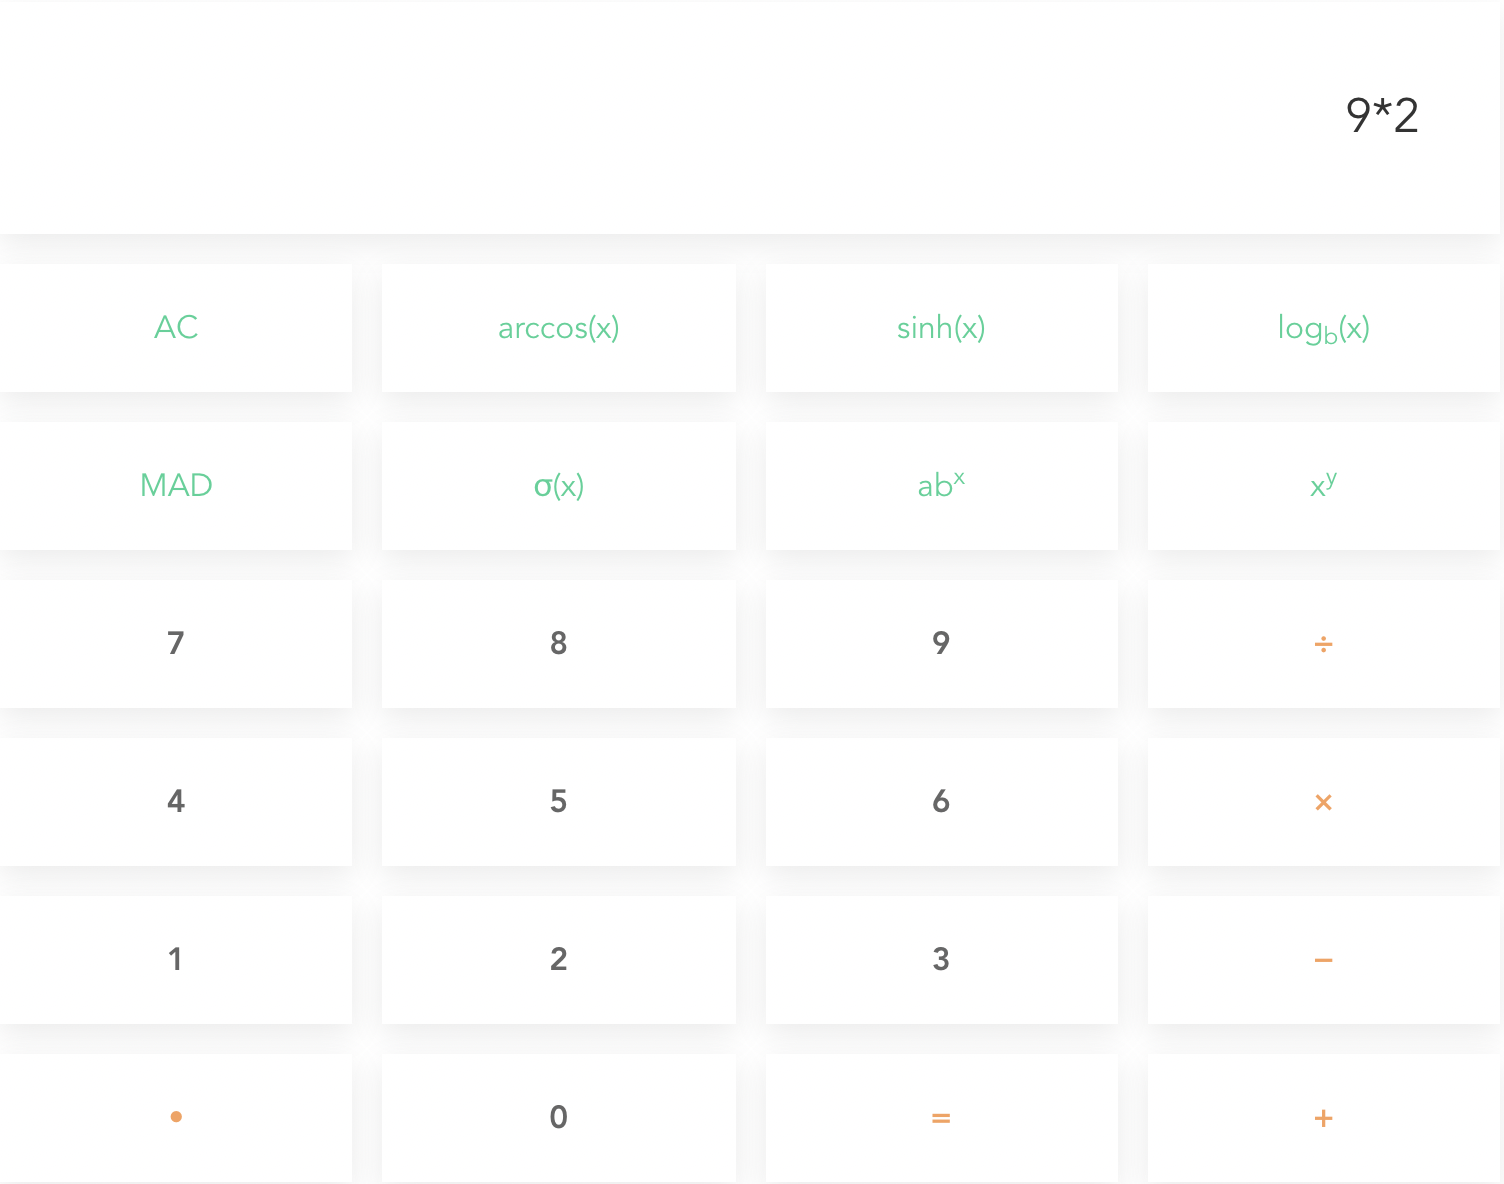
\includegraphics[width=0.70\linewidth]{images/calc.png}
    \end{center}
\end{frame}

\framecard[colorgreen]{{\color{white}\hugetext{Thank you!}}}

\end{document}